\section{Results}
\label{sec:results}

Table~\ref{tab:gates} summarises the acceptance gates; the subsections give the detail. All numbers are
taken from the run logs and evaluation files of the repository.

\begin{table*}[t]
\centering
\caption{Acceptance gates (fixed before training) and the measured values. ``Reduced'' marks runs whose
budget was cut (Table~\ref{tab:budget}).}
\label{tab:gates}
\small
\begin{tabular}{@{}llll@{}}
\toprule
benchmark & gate & measured & status\\
\midrule
A: Taylor--Green 2D & velocity rel.\ $L^2<10^{-4}$ & $4.05\times10^{-5}$ & passed\\
B: cavity, $\Rey=1000$ & Ghia $u$ and $v$ errors $<2\%$ & row C: 0.63\% / 2.05\%; row F: 19.8\% / 20.2\% & failed (see text: exact solution gives 2.29\% on $v$)\\
C: DFG 2D-2 cylinder (reduced) & $St$ within 3\% of 0.30, $C_{D,\max}$ within 5\% of 3.23 & \pending{St, Cd} & \pending{}\\
D: Taylor--Green 3D (reduced) & dissipation peak within 5\% of 0.01282 & \pending{peak} & \pending{}\\
inverse wake (reduced) & recover $\lambda_1=1$, $\lambda_2=0.01$ & \pending{} & \pending{}\\
PI-DeepONet (reduced) & zero-shot error at $\Rey=400$ $<10\%$ & \pending{} & \pending{}\\
\bottomrule
\end{tabular}
\end{table*}


\subsection{A: two-dimensional Taylor--Green vortex}
The full configuration (row G, stream-function output, 50k Adam steps and 1.2k L-BFGS iterations) reaches a
relative velocity error of $4.05\times10^{-5}$ ($u$: $4.17\times10^{-5}$, $v$: $3.93\times10^{-5}$) and a
pressure error of $2.59\times10^{-4}$ after the per-slice gauge alignment; the divergence is zero to machine
precision because of the stream-function form. The gate ($10^{-4}$) is passed with a factor 2.5 to spare.
Without the per-slice alignment, i.e.\ with a single constant for the whole space--time domain, the pressure
error of the same model would be reported as $3.3\times10^{-2}$, which illustrates how much of a
``pressure error'' can be gauge rather than physics. Training took about two hours at 0.139~s per step;
the trained network answers $3.9\times10^6$ velocity queries per second (stream-function velocities include one
derivative). Figure~\ref{fig:tgv2d} shows that the remaining error is spread uniformly over the domain at the
$10^{-5}$ level, without structure tied to the vortices.

\begin{figure}[t]
\centering
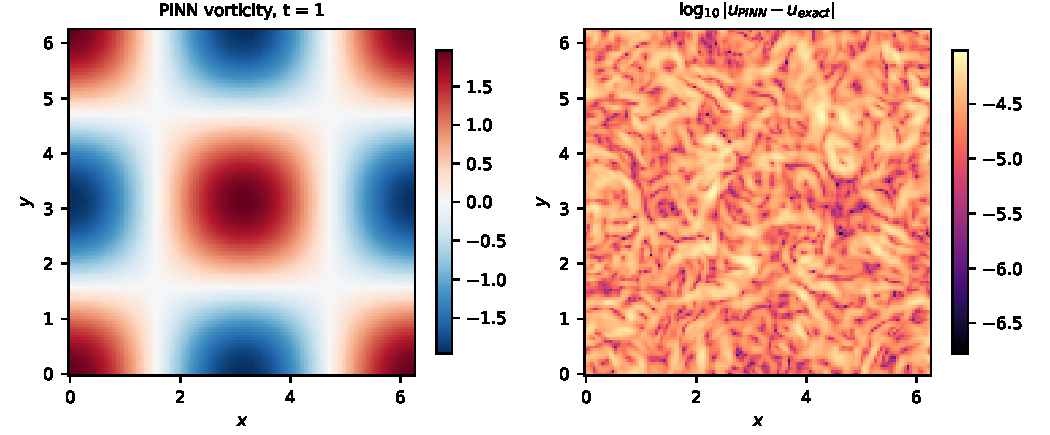
\includegraphics[width=\columnwidth]{figures/tgv2d.pdf}
\caption{Benchmark A at $t=1$: vorticity of the trained network (row G) and the pointwise magnitude of its
velocity error against the exact solution.}
\label{fig:tgv2d}
\end{figure}

\subsection{B: lid-driven cavity}
\label{sec:res-cavity}
Table~\ref{tab:cavity} collects the full-budget cavity runs and the reference solutions, all graded with the
same metric at $\Rey=1000$; Figure~\ref{fig:cavity} shows centreline profiles and divergence maps.

\begin{table*}[t]
\centering
\caption{Benchmark B at $\Rey=1000$, full budget (200k Adam steps over the curriculum, then up to 20k L-BFGS
iterations). Ghia errors are relative $L^2$ errors at the tabulated stations; ``vs FD'' is the relative $L^2$
error of the velocity field against the $512^2$ finite-difference solution of the same regularised-lid
problem. Where L-BFGS changed the result materially, both the end-of-Adam and the final value are given.}
\label{tab:cavity}
\small
\begin{tabular}{@{}lllcccc@{}}
\toprule
model & lid & weights & Ghia $u$ & Ghia $v$ & vs FD & wall-clock\\
\midrule
PINN row C (soft BC, earlier schedule$^{a}$) & soft & fixed & 0.38\% & 2.33\% & 0.12\% & 1.5 h Adam\\
PINN row C (soft BC) & soft & fixed & 0.63\% & 2.05\% & 0.27\% & 1.6 h\\
PINN row D, soft lid: end of Adam / after L-BFGS & soft lid & fixed & 1.04\% / 4.96\% & 2.20\% / 6.37\% & 1.9\% / 6.7\% & 3.3 h$^{b}$\\
PINN row F, soft lid (end of Adam$^{c}$) & soft lid & grad-norm & 16.0\% & 15.6\% & 21.0\% & 1.4 h Adam\\
PINN row D (hard lid) & hard & fixed & 21.3\% & 19.8\% & 28.3\% & 2.8 h\\
PINN row F (hard lid) & hard & grad-norm & 19.8\% & 20.2\% & 26.1\% & 2.3 h\\
\midrule
FD $512^2$, regularised lid & -- & -- & 0.41\% & 2.29\% & -- & --\\
FD $512^2$, unit lid & -- & -- & 0.89\% & 2.78\% & -- & --\\
JAX-PI reference field ($128^2$, unit lid) & -- & -- & 2.50\% & 1.76\% & -- & --\\
\bottomrule
\multicolumn{7}{@{}l}{\footnotesize $^{a}$ one learning-rate schedule decaying across all three curriculum stages (before the per-stage restart).}\\
\multicolumn{7}{@{}l}{\footnotesize $^{b}$ GPU shared with another workload during this run. $^{c}$ L-BFGS interrupted.}
\end{tabular}
\end{table*}

\begin{figure*}[t]
\centering
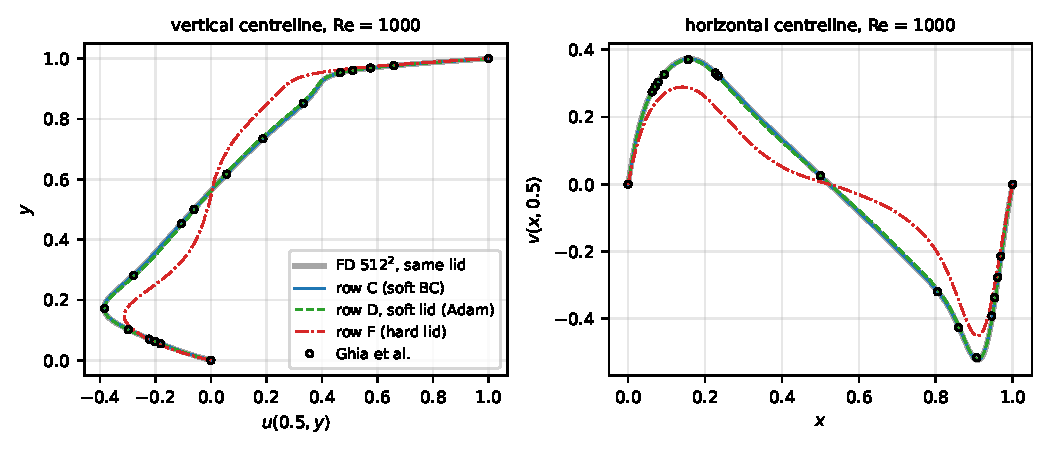
\includegraphics[width=0.49\textwidth]{figures/cavity_profiles.pdf}\hfill
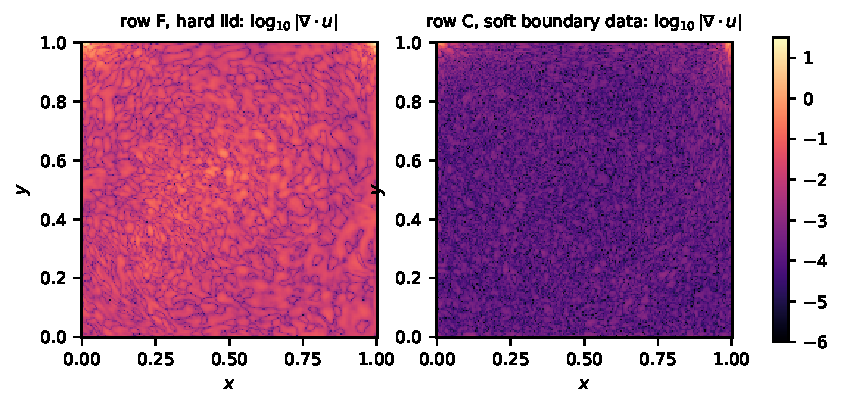
\includegraphics[width=0.49\textwidth]{figures/cavity_divergence.pdf}
\caption{Benchmark B at $\Rey=1000$. Left pair: centreline velocities of three PINN configurations against the
finite-difference solution of the same regularised-lid problem (grey) and the tables of Ghia et al.\ (circles);
the soft-boundary models lie on the FD curve. Right pair: divergence of the velocity for the fully hard lid
(row F) and for soft boundary data (row C); the hard lid leaves $|\nabla\cdot u|\sim10$ at the two top corners
and an unconverged interior.}
\label{fig:cavity}
\end{figure*}

\paragraph{The gate and the reference.} No run passes the 2\% gate on $v$, but the finite-difference
solutions show why the gate is not a useful measure at this level. As the grid is refined the unit-lid solution
converges to the spectral benchmark value of the primary vortex~\cite{botella1998} and moves \emph{away} from
Ghia's $v$ table (1.7\% at $128^2$, 2.1\% at $256^2$, 2.8\% at $512^2$); the converged regularised-lid solution
is 2.29\% from it. Station by station, Ghia's $v$ values next to the right wall are about 0.01 smaller in
magnitude than the converged fields. An exact solution of the benchmark as posed would therefore miss the gate
on $v$. Row C is 0.27\% from the converged field of its own problem, less than the 0.56\% by which the
$256^2$ and $512^2$ finite-difference fields differ from each other; its Ghia $v$ error (2.05\%) is below that of
the converged solution because its small errors partly compensate Ghia's near the wall. We report the gate
as missed, and regard the field error against the same-problem reference as the meaningful accuracy measure.

\paragraph{Which component fails.} The fully hard constraint breaks training whether the loss weights are
fixed (row D) or adapted (row F): in the $\Rey=1000$ stage the continuity loss does not settle below
$\sim10^{-2}$ (median $1.6\times10^{-2}$ for row D, between $1.5\times10^{-2}$ and $2.5\times10^{-1}$ for row F),
whereas row C drives the same term to $2\times10^{-8}$; the residual map shows the corner floor predicted in
Section~\ref{sec:method}, and the velocity field ends 26--28\% from the reference. Replacing the exact lid by a
loss term while keeping the other walls and $v$ exact (soft lid) restores the fixed-weight run to 1.9\% of
the reference field after Adam. With gradient-norm weighting the same soft lid fails again (21\%): the lid
term has small gradients, so its weight grows to about 465, which makes the soft lid effectively exact again,
while the continuity weight is lowered to about 0.2. On this problem the two components of rows D--G that
act on the boundary and on the loss weights are therefore harmful as specified, and the fully soft
configuration of row C is the most accurate.

\paragraph{L-BFGS on a fixed batch.} The second optimisation stage works on one fixed draw of 8192
collocation points. On the soft-lid row D it lowered that loss by three orders of magnitude (from
$2.6\times10^{-3}$ to $2.3\times10^{-6}$) and at the same time tripled the error of the field (1.9\% to 6.7\%): the
optimiser fits the chosen points, not the equations. On row C the stopping rule ended it after about 9k
iterations with no effect on the error. Refreshing the batch between L-BFGS restarts or using a much larger
fixed batch would be needed before the second stage can be trusted here.

\subsection{C: flow past a cylinder}
\label{sec:res-cylinder}
The first attempt followed the planned time marching with sixteen windows but only 4000 Adam steps per window.
After two windows (1~s of flow) it was stopped: the drag coefficient was 0.32 at $t=0.25$~s, 0.36 at 0.5~s and
0.45 at 0.75~s, an order of magnitude below the value of about 3.2 of the developed flow, and the front--rear
pressure difference was 0.19--0.29 instead of about 2.5. The continuity and momentum losses were still at
$2\times10^{-2}$ and $6\times10^{-3}$, the causal weights had not converged (minimum weight 0.92--0.94 with the
tolerance still at $\varepsilon=0.1$), and gradient-norm balancing had raised the weight of the outflow
condition on $v$ to 7000--9000 because its gradient is tiny. The drag integral itself is checked against
analytic fields in the test suite, so the low drag reflects a boundary layer and near wake that the network had
not yet resolved. Continuing would have propagated this state through fourteen more windows and could not
produce the shedding needed for a Strouhal number, so the same GPU time was spent on four windows of 12k steps.

\pending{cylinder_G_4x12k results: Cd, Cl, dP per window, causal convergence; row E comparison if run;
gate status; figure.}

\subsection{D: three-dimensional Taylor--Green vortex}
\label{sec:res-tgv3d}
\pending{tgv3d_H: E_k(0) vs 1/8, dissipation peak and time vs 0.01282 at 9.00, enstrophy-based peak,
spectrum slope; figure energy/dissipation/spectrum + a movie frame.}

\subsection{Inverse problem}
\label{sec:res-inverse}
\pending{lambda_1, lambda_2, errors, hidden-pressure error, velocity errors.}

\subsection{Parametric surrogate}
\label{sec:res-deeponet}
\pending{zero-shot at Re=400, errors at 100 and 1000, inference time for a new Re.}

\subsection{Ablation}
\label{sec:res-ablation}
\pending{table of rows A-G on A and B: rel L2 + steps to target; figure ablation.pdf.}

\subsection{Cost}
\label{sec:res-cost}
\pending{table: training wall-clock, step time, peak memory, inference throughput for every run.}

